\scanpage{54}
\mspage{\handwritten{22}}
% archive sheet number: 53

\uline{Theorem \handwritten{11.16}.}- (Chevalley). \unsure{Soeent|Let} $k$ be a field, $G$ an affine algebraic $k$-group, $H$ a closed subgroup prescheme of $G$. Then there exist finitely many linearly independent elements $a_i$ of the algebra $A$ of $G$, such that $H$ is the largest closed subgroup prescheme of $G$ under which the $a_i$ are semi-invariants; one may moreover suppose that all the $a_i$ have the same \deleted{associated character (hence the same} weight\deleted{)} under $H$.

Recall that, since $G$ is affine, the same is true of $H$ (\deleted{Lecture} I 4.2.3). Let $A$ (resp. $B$) be the algebra of $G$ (resp. $H$); by \deleted{\handwritten{§}}EGA I 4.2.3, there is an ideal $I$ of $A$ such that $B$ \unsure{qoit|is} isomorphic to $A/I$\begin{tikzpicture}[x=1cm,y=1cm,baseline=(n.base)]\node[inner sep=0pt] (n) at (0,0) {.};\draw[thin] (-.08,-.07)--(.09,.32);\end{tikzpicture} Since $G$ acts on itself by left translations, it also acts on $A$, this action being expressed by the diagonal map $\handwritten{\Delta}:A\handwritten{\longrightarrow}A\handwritten{\otimes}_k A$ (\deleted{Lecture} I 4.2 and 4.7.2). Since $G$ is of finite type over $k$, $A$ is of finite type over $k$, hence $I$ \deleted{\unsure{ad}} admits a finite system of generators $(g_1,\ldots,g_r)$. It follows from (11.9) that there is a finite-dimensional vector subspace $V$ of $A$ \deleted{sat} stable under $G$, and containing each of the $g_i$.

\margin{\figure{\handwritten{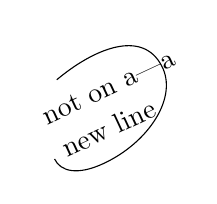
\begin{tikzpicture}[x=0.45cm,y=0.45cm]\draw[rotate=25] (-1,1.3) .. controls (.3,1.65) and (1.8,1.6) .. (1.85,.4) .. controls (1.9,-.6) and (.6,-1.4) .. (-.8,-1.4) .. controls (-1.6,-1.4) and (-2,-1.1) .. (-2,-.7);\node[rotate=25] at (0,0.55) {not on \unsure{a|a}};\node[rotate=25] at (0,-0.6) {new line};\end{tikzpicture}}}}
\margin{\figure{\handwritten{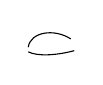
\begin{tikzpicture}[x=0.3cm,y=0.3cm]\draw (1,.8) .. controls (.3,1.25) and (-.7,1.1) .. (-.8,.45);\draw (-.8,.25) .. controls (-.4,.05) and (.4,.1) .. (1.15,.3);\end{tikzpicture}}}}
Put then $W=V\handwritten{\cap}I$, it is a finite-dimensional vector space over $k$, whose dimension we shall denote by $d$. Since $V$ contains all the $g_i$, $W$ generates \deleted{the algebra}\inserted{\handwritten{the ideal}} $I$.

\margin{\figure{\handwritten{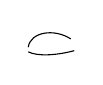
\begin{tikzpicture}[x=0.3cm,y=0.3cm]\draw (1,.8) .. controls (.3,1.25) and (-.7,1.1) .. (-.8,.45);\draw (-.8,.25) .. controls (-.4,.05) and (.4,.1) .. (1.15,.3);\end{tikzpicture}}}}
Write $p:A\handwritten{\longrightarrow}A/I=B$ for the canonical map, and $q=p\handwritten{\otimes}\operatorname{id}_A:A\handwritten{\otimes}_k A\handwritten{\longrightarrow}(A/I)\handwritten{\otimes}_k A$ Then the action of $H$ on $A$ is determined by $q\mathbin{o}\handwritten{\Delta}:A\handwritten{\longrightarrow}B\handwritten{\otimes}_k A$. Since $H$ is a subgroup prescheme of $G$, the diagonal map $A/I\handwritten{\longrightarrow}(A/I)\handwritten{\otimes}_k(A/I)=((A/I)\handwritten{\otimes}_k A)/((A/I)\handwritten{\otimes}_k I)$ is obtained from $q\mathbin{o}\handwritten{\Delta}$ by passage to the quotient, which shows that $(q\mathbin{o}\handwritten{\Delta})(I)\subset(A/I)\handwritten{\otimes}_k I$, in other \linebreak words, $I$ is stable under $H$. Since $V$ is stable under $G$, hence under $H$, we see that $W$ is stable under $H$.

Put $E=\handwritten{\wedge}^d V$, let $(w_1,\ldots,w_d)$ be a basis of $W$ over $k$, and let $(e_{\unsure{o|0}},\mathinner{..},e_n)$ be a basis of $E$ over $k$ containing $e_{\unsure{o|0}}=w_1\handwritten{\wedge}\cdots\handwritten{\wedge}w_d$. The action of $G$ on $\handwritten{V}$ canonically determines an action of $G$ on $\handwritten{\wedge}^d V$, which defines a linear map $\handwritten{\rho}:E\handwritten{\longrightarrow}A\handwritten{\otimes}_k E$. Put $\handwritten{\rho}(e_i)=\handwritten{\sum}a_j^i\handwritten{\otimes}e_j$, and $a_i=a_i^{\unsure{o|0}}$. Since $W$ is stable under $H$, if we put \margin{\figure{\begin{tikzpicture}[x=1cm,y=1cm]\draw[thin] (0,.02)--(.18,-.01);\end{tikzpicture}}}$\handwritten{\sigma}=(p\handwritten{\otimes}\operatorname{id}_E)\mathbin{o}\handwritten{\rho}:E\handwritten{\longrightarrow}(A/I)\handwritten{\otimes}_k E$, it is clear that $\handwritten{\sigma}(e_{\unsure{o|0}})$ is proportional to $e_{\unsure{o|0}}$, in other words, for $1\leqq i\leqq n$, we have $a_i\in I$. The axio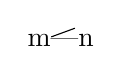
\begin{tikzpicture}[x=1cm,y=1cm,baseline=(a.base)]\node[inner sep=0pt] (a) at (0,0) {\unsure{m|n}};\draw (-.12,.05)--(.18,.16);\end{tikzpicture} (CM1) of (\deleted{Lecture} I 4.7.2) applied to
